\section{Linux Application Stack}

\begin{frame}
  \frametitle{User/Kernel mode}
  \begin{itemize}
    \item User mode vs Kernel mode are often used to refer to the privilege
          level of execution.
    \item This mode actually refers to the processor execution mode which is a
          hardware mode.
    \begin{itemize}
      \item Might be named differently between architectures but the goal is
            the same
    \end{itemize}
    \item Allows the kernel to control the full processor state (handle
      exceptions, MMU, etc) whereas the userspace can only do basic control
          and execute under the kernel supervision.
  \end{itemize}
\end{frame}

\begin{frame}
  \frametitle{Processes and Threads (1/2)}
  \begin{itemize}
    \item A process is a group of resources that are allocated by the operating
          to allow the execution of a program.
    \begin{itemize}
      \item Memory regions, threads, files, etc.
    \end{itemize}
    \item A process is identified by a PID ({\bf P}rocess {\bf ID}) and all the
          information that are specific to this process are exposed in
          \code{/proc/<pid>}.
    \begin{itemize}
      \item A special file named \code{/proc/self} accessible by the process
            points to the proc folder associated to it.
    \end{itemize}
    \item When starting a process, it initially has one execution thread that
          is represented by a \kstruct{task_struct} and that can be scheduled.
    \begin{itemize}
      \item A process is represented in the kernel by a thread associated to
            multiple resources.
    \end{itemize}
  \end{itemize}
\end{frame}

\begin{frame}
  \frametitle{Processes and Threads (2/2)}
  \begin{itemize}
    \item Threads are independent execution units that are sharing common
          resources inside a process.
    \begin{itemize}
      \item Same address space, file descriptors, etc.
    \end{itemize}
    \item A new process is created using the fork() system call
          (\manpage{fork}{2}) and a new thread is created using
          \code{pthread_create()} (\manpage{pthread_create}{3}).
    \begin{itemize}
      \item Internally, both will call \code{clone()} with different flags
    \end{itemize}
    \item At any moment, only one task is executing on a CPU core and is
          accessible using \kfunc{get_current} function (defined by
          architecture and often stored in a register).
    \item Each CPU core will execute a different task.
    \item A task can only be executing on one core at a time.
  \end{itemize}
\end{frame}

\begin{frame}
  \frametitle{MMU and memory management}
  \begin{itemize}
    \item Under Linux Kernel (when using \kconfigval{CONFIG_MMU}{y}), all addresses
          that are accessed by the CPU are virtual
    \item The Memory Management Unit allows to map these virtual addresses to
          physical memory (either RAM or IO)
    \item All these mappings are inserted into the page table that is used by the
          MMU hardware to translate the CPU access to virtual addresses
    \item The MMU allows to restrict access to the page mappings via some
          attributes
    \begin{itemize}
      \item No Execute, Writable, Readable bits, Privileged/User bit, cacheability
    \end{itemize}
    \item The MMU base unit for mappings is called a page
    \item Page size is fixed and depends on the architecture/kernel
          configuration.
  \end{itemize}
\end{frame}

\begin{frame}
  \frametitle{Userspace/Kernel memory layout}
  \begin{columns}
    \column{0.55\textwidth}
    \begin{itemize}
      \item Each process has its own set of virtual memory areas (\code{mm}
            field of \kstruct{task_struct}).
      \item Also have their own page table
      \begin{itemize}
        \item But share the same kernel mappings
      \end{itemize}
      \item By default, all user mapping addresses are randomized to
            minimize attack surface (base of heap, stack, text, data, etc).
      \begin{itemize}
        \item {\bf A}ddress {\bf S}pace {\bf L}ayout {\bf R}andomization
        \item Can be disabled using \code{norandmaps} command line parameter
      \end{itemize}
    \end{itemize}
    \column{0.45\textwidth}
    \includegraphics[height=0.8\textheight]{slides/debugging-linux-application-stack/memory_layout.pdf}
  \end{columns}
\end{frame}

\begin{frame}
  \frametitle{Userspace/Kernel memory layout}
  Multiple processes have different user memory spaces
  \center\includegraphics[height=0.7\textheight]{slides/debugging-linux-application-stack/multiple_process.pdf}
\end{frame}

\begin{frame}[fragile]
  \frametitle{Kernel memory map}
  \begin{columns}
    \column{0.55\textwidth}
    \begin{itemize}
      \item The kernel has it own memory mapping.
      \item Linear mapping is setup at kernel startup by inserting all the
            entries in the kernel init page table.
      \item Multiple areas are identified and their location differs between the
            architectures.
      \item {\bf K}ernel {\bf A}ddress {\bf S}pace {\bf L}ayout
            {\bf R}andomization also allows to randomize kernel address space
            layout.
      \begin{itemize}
        \item Can be disabled using \code{nokaslr} command line parameter
      \end{itemize}
    \end{itemize}
    \column{0.45\textwidth}
    \includegraphics[height=0.8\textheight]{slides/debugging-linux-application-stack/kernel_layout.pdf}
  \end{columns}
\end{frame}

\begin{frame}[fragile]
  \frametitle{Userspace memory segments}
  \begin{itemize}
    \item When starting a process, the kernel sets up a number of various memory
          segments (named VMAs and backed by \kstruct{vma}) that have
          different execution attributes.
    \item VMA are actually memory zones that are mapped with specific
          attributes (R/W/X).
    \item A segmentation fault happens when a program tries to access a non
          existent VMA or a correct one but in a way that is not allowed.
    \begin{itemize}
      \item Writing data in a read-only segment
      \item Executing data from a non-executable segment
    \end{itemize}
    \item New memory zones can be created using \code{mmap()}
          (\manpage{mmap}{2})
    \item Per application mappings are visible in {\em /proc/<pid>/maps}\\
    \begin{minted}[fontsize=\small]{console}
7f1855b2a000-7f1855b2c000 rw-p 00030000 103:01 3408650  ld-2.33.so
7ffc01625000-7ffc01646000 rw-p 00000000 00:00 0         [stack]
7ffc016e5000-7ffc016e9000 r--p 00000000 00:00 0         [vvar]
7ffc016e9000-7ffc016eb000 r-xp 00000000 00:00 0         [vdso]
    \end{minted}
  \end{itemize}
\end{frame}

\begin{frame}[fragile]
  \frametitle{Userspace memory types}
  \center \includegraphics[height=0.7\textheight]{slides/debugging-linux-application-stack/mem_type.pdf}
\end{frame}

\begin{frame}[fragile]
  \frametitle{Terms for memory in Linux tools}
  \begin{itemize}
    \item When using Linux tools, four terms are used to describe memory:
    \begin{itemize}
      \item {\em VSS/VSZ}: Virtual Set Size (Virtual memory size, shared libraries
            included).
      \item {\em RSS}: Resident Set Size (Total physical memory usage, shared
            libraries included).
      \item {\em PSS}: Proportional Set Size (Actual physical memory used, divided
            by the number of times it has been mapped).
      \item {\em USS}: Unique Set Size (Physical memory occupied by the process,
            shared mappings memory excluded).
    \end{itemize}
    \item VSS >= RSS >= PSS >= USS.
  \end{itemize}
\end{frame}

\begin{frame}
  \frametitle{Process context}
  \begin{itemize}
    \item The \emph{process context} can be seen as the content of
    the CPU registers associated to a process: execution register, stack register...
    \item This context also designates an execution state and allows to sleep
          inside kernel mode.
    \item A process that is executing in process context can be preempted.
    \item While executing in such context, the current process
          \kstruct{task_struct} can be accessed using \kfunc{get_current}.
  \end{itemize}
  \vspace{0.5cm}
  \includegraphics[height=0.2\textheight]{slides/debugging-linux-application-stack/process_context.pdf}
\end{frame}

\begin{frame}[fragile]
  \frametitle{Scheduling}
  \begin{itemize}
    \item The scheduler can be invoked for various reasons
    \begin{itemize}
      \item On a periodic tick caused by interrupt (\kconfig{HZ})
      \item On a programmed interrupt on tickless systems (\kconfigval{CONFIG_NO_HZ}{y})
      \item Voluntarily by calling \kfunc{schedule} in code
      \item Implicitly by calling functions that can sleep (blocking
            operations such as \kfunc{kmalloc}, \kfunc{wait_event}).
    \end{itemize}
    \item When entering the schedule function, the scheduler will elect a new
          \kstruct{task_struct} to run and will eventually call the
          \kfunc{switch_to} macro.
    \item \kfunc{switch_to} is defined by architecture code and it will save
          the current task process context and restore the one of the next task
          to be run while setting the new current task running.
  \end{itemize}
\end{frame}

\begin{frame}
	\frametitle{The Linux Kernel Scheduler}
	\begin{itemize}
		\item The Linux Kernel Scheduler is a key piece in having a real-time behaviour
		\item It is in charge of deciding which \textbf{runnable} task gets executed
		\item It also elects on which CPU the task runs, and is tightly coupled to CPUidle and CPUFreq
		\item It schedules both \textbf{userspace} tasks and \textbf{kernel} tasks
		\item Each task is assigned one \textbf{scheduling class} or \textbf{policy}
		\item The class determines the algorithm used to elect each task
		\item Tasks with different scheduling classes can coexist on the system
	\end{itemize}
\end{frame}

\begin{frame}
	\frametitle{Non-Realtime Scheduling Classes}
	There are 3 \textbf{Non-RealTime} classes
	\begin{itemize}
		\item \code{SCHED_OTHER}: The default policy, using a time-sharing algorithm
		\item \ksym{SCHED_BATCH}: Similar to \code{SCHED_OTHER}, but designed for CPU-intensive loads that affect the wakeup time
		\item \ksym{SCHED_IDLE}: Very low priority class. Tasks with this policy will run only if nothing else needs to run.
		\item \code{SCHED_OTHER} and \ksym{SCHED_BATCH} use the \textbf{nice} value to increase or decrease their scheduling frequency
		\begin{itemize}
			\item A higher nice value means that the tasks gets scheduled \textbf{less} often
		\end{itemize}
	\end{itemize}
\end{frame}

\begin{frame}
	\frametitle{Realtime Scheduling Classes}
	There are 3 \textbf{Realtime} classes
	\begin{itemize}
		\item Runnable tasks will preempt any other lower-priority task
		\item \ksym{SCHED_FIFO}: All tasks with the same priority are scheduled \textbf{First in, First out}
		\item \ksym{SCHED_RR}: Similar to \ksym{SCHED_FIFO} but with a time-sharing round-robin between tasks with the same priority
		\item Both \ksym{SCHED_FIFO} and \ksym{SCHED_RR} can be assigned a priority between 1 and 99
		\item \ksym{SCHED_DEADLINE}: For tasks doing recurrent jobs, extra attributes are attached to a task
			\begin{itemize}
				\item A computation time, which represents the time the task needs to complete a job
				\item A deadline, which is the maximum allowable time to compute the job
				\item A period, during which only one job can occur
			\end{itemize}
		\item Using one of these classes is necessary but not sufficient to get real-time behavior
	\end{itemize}
\end{frame}

\begin{frame}
	\frametitle{Changing the Scheduling Class}
	\begin{itemize}
		\item The Scheduling Class is set per-task, and defaults to \code{SCHED_OTHER}
		\item The \manpage{sched_setscheduler}{2} syscall allows changing the class of a task
		\item The \code{chrt} tool uses it to allow changing the class of a running task:
			\begin{itemize}
				\item \code{chrt -f/-b/-o/-r/-d -p PRIO PID}
			\end{itemize}
		\item It can also be used to launch a new program with a dedicated class:
			\begin{itemize}
				\item \code{chrt -f/-b/-o/-r/-d PRIO CMD}
			\end{itemize}
		\item New processes will inherit the class of their parent except if the \ksym{SCHED_RESET_ON_FORK} flag is set with \manpage{sched_setscheduler}{2}
		\item See \manpage{sched}{7} for more information
	\end{itemize}
\end{frame}


\begin{frame}
  \frametitle{Context switching}
  \begin{itemize}
    \item Context switching is the action of changing the execution mode of the
          processor (Kernel $\leftrightarrow$ User).
    \begin{itemize}
      \item Explicitly by executing system calls instructions (synchronous
            request to the kernel from user mode).
      \item Implicitly when receiving exceptions (MMU fault, interrupts,
            breakpoints, etc).
    \end{itemize}
    \item This state change will end up in a kernel entrypoint (often call vectors)
          that will execute necessary code to setup a correct state for kernel
          mode execution.
    \item The kernel takes care of saving registers, switching to the kernel
          stack and potentially other things depending on the architecture.
    \begin{itemize}
      \item Does not use the user stack but a specific kernel fixed size stack
            for security purposes.
    \end{itemize}
  \end{itemize}
\end{frame}


\begin{frame}
  \frametitle{Exceptions}
  \begin{itemize}
    \item Exceptions designate the kind of events that will trigger a CPU
          execution mode change to handle the exception.
    \item Two main types of exceptions exist: synchronous and asynchronous.
    \begin{itemize}
      \item Asynchronous exceptions when a fault happens while executing (MMU,
            bus abort, etc) or when an interrupt is received (either software
            or hardware).
      \item Synchronous when executing some specific instructions (breakpoint,
            syscall, etc)
    \end{itemize}
    \item When such exception is triggered, the processor will jump to the
          exception vector and execute the code that was setup for this
          exception.
  \end{itemize}
\end{frame}

\begin{frame}
  \frametitle{Interrupts}
  \begin{itemize}
    \item Interrupts are asynchronous signals that are generated by the hardware
          peripherals.
    \begin{itemize}
      \item Can also be synchronous when generated using a specific instruction
            ({\bf I}nter {\bf P}rocessor {\bf I}nterrupts for instance).
    \end{itemize}
    \item When receiving an interrupt, the CPU will change its execution mode by
          jumping to a specific vector and switching to kernel mode to handle the
          interrupt.
    \item When multiple CPUs (cores) are present, interrupts are often directed
          to a single core.
    \item This is called "IRQ affinity" and it allows to control the IRQ load for
          each CPU
    \begin{itemize}
      \item See \kdochtml{core-api/irq/irq-affinity} and
            \href{https://linux.die.net/man/1/irqbalance}{man irqbalance(1)}
    \end{itemize}
  \end{itemize}
\end{frame}

\begin{frame}
  \frametitle{Interrupts}
  \begin{itemize}
    \item While handling the interrupts, it is executing in a specific context
          named {\em interrupt context}.
    \item This context does not have access to userspace and should not use
          \kfunc{get_current}.
    \item Depending on the architecture, might use an IRQ stack.
    \item Interrupts are disabled (no nested interrupt support)!
  \end{itemize}
  \begin{center}
    \includegraphics[height=0.2\textheight]{slides/debugging-linux-application-stack/interrupt_context.pdf}
  \end{center}
\end{frame}

\begin{frame}[fragile]
  \frametitle{System Calls (1/2)}
  \begin{itemize}
    \item A system call allows the user space to request services from the
          kernel by executing a special instruction that will switch to the
          kernel mode (\manpage{syscall}{2})
    \begin{itemize}
      \item When executing functions provided by the libc (\code{read()},
            \code{write()}, etc), they often end up executing a system call.
    \end{itemize}
    \item System calls are identified by a numeric identifier that is passed
          via the registers.
    \begin{itemize}
      \item The kernel exports some defines (in \code {unistd.h}) that are named
            \code{__NR_<sycall>} and defines the syscall identifiers.
    \end{itemize}
  \end{itemize}
  \begin{block}{}
    \begin{minted}[fontsize=\small]{C}
#define __NR_read 63
#define __NR_write 64
    \end{minted}
  \end{block}
\end{frame}

\begin{frame}[fragile]
  \frametitle{System Calls (2/2)}
  \begin{itemize}
    \item The kernel holds a table of function pointers which matches these
          identifiers and will invoke the correct handler after checking the
          validity of the syscall.
    \item System call parameters are passed via registers (up to 6).
    \item When executing this instruction the CPU will change its execution
    state and switch to the kernel mode.
    \item Each architecture uses a specific hardware mechanism
    (\manpage{syscall}{2})
  \end{itemize}
  \begin{block}{}
    \begin{minted}[fontsize=\small]{asm}
    mov w8, #__NR_getpid
    svc #0
    tstne x0, x1
    \end{minted}
  \end{block}
\end{frame}

\begin{frame}[fragile]
  \frametitle{Kernel execution contexts}
  \begin{itemize}
    \item The kernel runs code in various contexts depending on the event it is
          handling.
    \item Might have interrupts disabled, specific stack, etc.
  \end{itemize}
\end{frame}

\begin{frame}[fragile]
  \frametitle{Kernel threads}
  \begin{itemize}
    \item Kernel threads (kthreads) are a special kind of \kstruct{task_struct} that do not
          have any user resources associated (\code{mm == NULL}).
    \item These processes are cloned from the \code{kthreadd} process and can be
          created using \kfunc{kthread_create}.
    \item Kernel threads are scheduled and are allowed to sleep much like a
          process executing in process context.
    \item Kernel threads are visible and their names are displayed between
          brackets under {\em ps}:
  \end{itemize}
  \begin{block}{}
    \begin{minted}[fontsize=\tiny]{console}
$ ps --ppid 2 -p 2 -o uname,pid,ppid,cmd,cls
USER         PID    PPID CMD                         CLS
root           2       0 [kthreadd]                   TS
root           3       2 [rcu_gp]                     TS
root           4       2 [rcu_par_gp]                 TS
root           5       2 [netns]                      TS
root           7       2 [kworker/0:0H-events_highpr  TS
root          10       2 [mm_percpu_wq]               TS
root          11       2 [rcu_tasks_kthread]          TS
    \end{minted}
  \end{block}
\end{frame}

\begin{frame}
  \frametitle{Workqueues}
  \begin{itemize}
    \item Workqueues allows to schedule some work to be executed at some point
          in the future
    \item Workqueues are executing the work functions in kernel threads.
    \begin{itemize}
      \item Allows to sleep while executing the defered work.
      \item Interrupts are enabled while executing
    \end{itemize}
    \item Work can be executed either in dedicated work queues or in the
          default workqueue that is shared by multiple users.
  \end{itemize}
\end{frame}

\begin{frame}
  \frametitle{softirq}
  \begin{itemize}
    \item SoftIRQs is a specific kernel mecanism that is executed in
          software interrupt context.
    \item Allows to execute code that needs to be defered after interrupt
          handling but needs low latency.
    \begin{itemize}
      \item Executed right after hardware IRQ have been handled in interrupt
            context.
      \item Same context than executing interrupt handler so sleeping is not
            allowed.
    \end{itemize}
    \item Tasklets are using softirqs to execute their work so they run in the
          same context and the same constraints are applied.
  \end{itemize}
\end{frame}

\begin{frame}
  \frametitle{Interrupts \& Softirqs}
  \includegraphics[height=6cm]{slides/debugging-linux-application-stack/softirqs.pdf}
\end{frame}

\begin{frame}
  \frametitle{Threaded interrupts}
  \begin{itemize}
    \item Threaded interrupts are a mecanism that allows to handle the interrupt
          using a hard IRQ handler and a threaded IRQ handler.
    \item A threaded IRQ handler will allow to execute work that can potentially
          sleep in a kthread.
    \item One kthread is created for each interrupt line that was requested as
          a threaded IRQ.
    \begin{itemize}
      \item {\em kthread} is named \code{irq/<irq>-<name>} and can be seen using {\em ps}.
    \end{itemize}
  \end{itemize}
\end{frame}

\begin{frame}
  \frametitle{Allocations and context}
  \begin{itemize}
    \item Allocating memory in the kernel can be done using multiple functions:
    \begin{itemize}
      \item \mint{c}+void *kmalloc(size_t size, int flags);+
      \item \mint{c}+void *kzalloc(size_t size, gfp_t flags);+
      \item \mint{c}+unsigned long __get_free_pages(int flags, unsigned int order)+
    \end{itemize}
    \item All allocation functions take a flags parameter which allows to
          designate the kind of memory that is needed.
    \begin{itemize}
      \item \ksym{GFP_KERNEL}: Normal allocation, can sleep while allocating
            memory (can not be used in interrupt context).
      \item \ksym{GFP_ATOMIC}: Atomic allocation, won't sleep while allocating
            data.
    \end{itemize}
  \end{itemize}
\end{frame}

\begin{frame}
  \frametitle{ELF files}
    \begin{columns}
      \column{0.75\textwidth}
      {\bf E}xecutable and {\bf L}inkable {\bf F}ormat
      \begin{itemize}
        \item File starting with a header which holds binary structures
              defining the file
        \item Collection of segments and sections that contain data
        \begin{itemize}
          \item \code{.text} section: Code
          \item \code{.data} section: Data
          \item \code{.rodata} section: Read-only Data
          \item \code{.debug_info} section: Contains debugging information
        \end{itemize}
        \item Sections are part of a segment which can be loadable in memory
        \item Same format for all architectures supported by the kernel and also
              \code{vmlinux} format
        \begin{itemize}
          \item Also used by a lot of other operating systems as the standard
                executable file format
        \end{itemize}
      \end{itemize}
      \column{0.25\textwidth}
      \vspace{0.5cm}
      %% Source: https://commons.wikimedia.org/wiki/File:Elf-layout--en.svg
      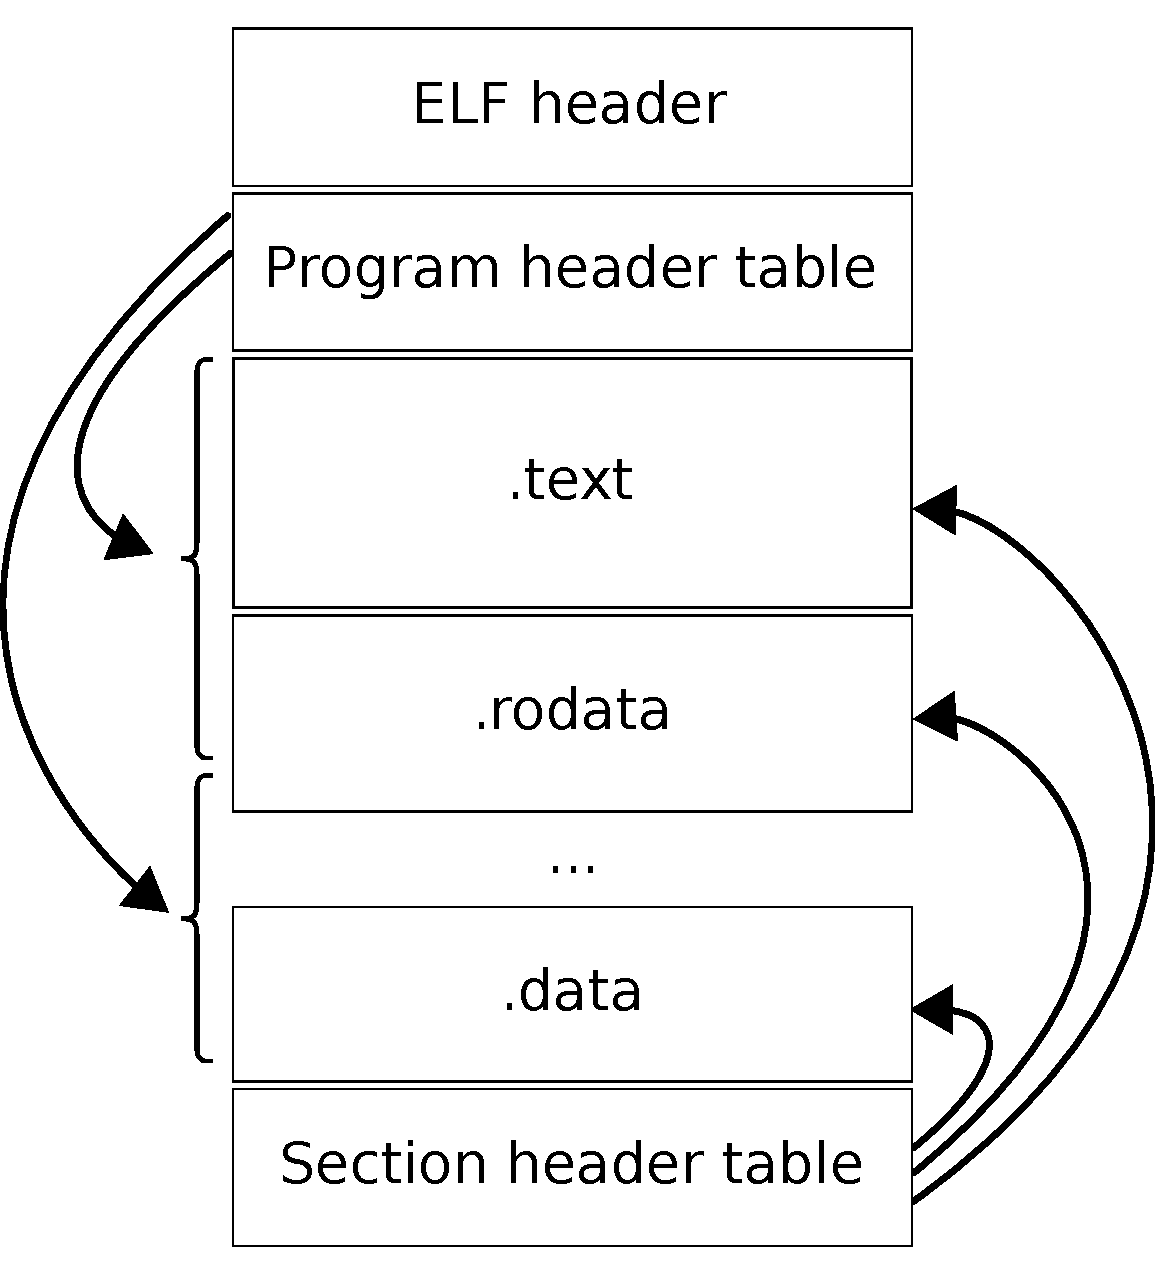
\includegraphics[height=0.5\textheight]{slides/debugging-linux-application-stack/elf_layout.pdf}
    \end{columns}
  \end{frame}

\begin{frame}[fragile]
  \frametitle{Debugging with ELF files}
  \begin{columns}
    \column{0.75\textwidth}
    \begin{itemize}
      \item GDB uses ELF files since they are containing the debugging information
      \item Debugging information uses the DWARF format
      \item Allows the debugger to match addresses and symbol names, call
            sites, etc
      \item Debugging information is generated by GDB and included in the
            ELF file when compiled with \code{-g}
      \begin{itemize}
        \item \code{-g1}: minimal debug information (enough for backtraces)
        \item \code{-g2}: default debug level when using \code{-g}
        \item \code{-g3}: includes extra debugging information (macro
          definitions)
      \end{itemize}
      \item See \href{https://gcc.gnu.org/onlinedocs/gcc/Debugging-Options.html}{GCC documentation}
        about debugging for more information
    \end{itemize}
    \column{0.25\textwidth}
    
\includegraphics[height=0.3\textheight]{slides/debugging-linux-application-stack/dwarf_logo.jpg}
  \end{columns}
\end{frame}

\begin{frame}[fragile]
  \frametitle{Debugging with compiler optimizations}
  \begin{itemize}
    \item Compiler optimizations (\code{-O<level>}) can lead to optimizing out some variables
          and function calls.
    \item Trying to display them with GDB will display
    \begin{itemize}
      \item \code{$1 = <value optimized out>}
    \end{itemize}
    \item If one wants to inspect variables and functions, it is possible to
          compile the code using \code{-O0} (no optimization).
    \begin{itemize}
      \item {\em Note: The kernel can only be compiled with \code{-O2} or \code{-Os}}
    \end{itemize}
    \item It is also possible to annotate function with compiler attributes:
    \begin{itemize}
      \item \code{__attribute__((optimize("O0")))}
    \end{itemize}
    \item Remove function \code{static} qualifier to avoid inlining the function
    \begin{itemize}
      \item {\em Note: LTO (Link Time Optimization) can defeat this.}
    \end{itemize}
    \item Set a specific variable as \code{volatile} to prevent the compiler
          from optimizing it out.
  \end{itemize}
\end{frame}

\begin{frame}
  \frametitle{Shared libraries}
  \begin{itemize}
    \item Shared libraries are provided as {\em .so} files that are actually ELF files
    \begin{itemize}
      \item Loaded at startup by \code{ld.so} (the dynamic loader)
      \item Or at runtime using \code{dlopen()} from your code
    \end{itemize}
    \item When starting a program (an ELF file actually), the kernel will
          parse it and load the interpreter that needs to be invoked.
    \begin{itemize}
      \item Most of the time \code{PT_INTERP} program header of the ELF file is
            set to \code{ld-linux.so}.
    \end{itemize}
    \item At loading time, the dynamic loader \code{ld.so} will resolve all the
          symbols that are present in dynamic libraries.
    \item Shared libraries are loaded only once by the OS and then mappings are
          created for each application that uses the library.
    \begin{itemize}
      \item This allows to reduce the memory used by libraries.
    \end{itemize}
  \end{itemize}
\end{frame}

\begin{frame}
  \frametitle{Kernel debug features}
  \begin{itemize}
    \item The kernel contains multiple mechanisms to analyze functions calls,
          arguments, hook specific handlers and much more
    \begin{itemize}
      \item {\em ptrace} allows tracing another process
      \item {\em kprobes} can hook handlers on almost any code site
      \item {\em ftrace} allows tracing functions using different tracers
      \item {\em eBPF} is a powerful framework in the kernel allowing to use BPF
            language in sandboxed environments and execute complex actions and
            data gathering
    \end{itemize}
    \item Some debug features use the {\em debugfs} filesystem to expose their
          functionalities.
    \begin{itemize}
      \item \codewithhash{\# mount -t debugfs none /sys/kernel/debug/}
    \end{itemize}
  \end{itemize}
\end{frame}

\begin{frame}[fragile]
  \frametitle{ptrace}
  \begin{itemize}
    \item The {\em ptrace} mechanism allows processes to trace other processes by
          accessing tracee memory and register contents
    \item A tracer can observe and control the execution state of another
          process
    \item Works by attaching to a tracee process using the \code{ptrace()}
          system call (see \manpage{ptrace}{2})
    \item Can be executed directly using the \code{ptrace()} call but often used
          indirectly using other tools.
  \end{itemize}

  \begin{block}{}
    \begin{minted}[fontsize=\small]{C}
long ptrace(enum __ptrace_request request, pid_t pid, void *addr, void *data);
    \end{minted}
  \end{block}

  \begin{itemize}
    \item Used by {\em GDB}, {\em strace} and all debugging tools that need access to the
          tracee process state
  \end{itemize}
\end{frame}
